% \newcommand{\baselineEvalFigure}{
% \begin{figure}[t]
%     \centering
%     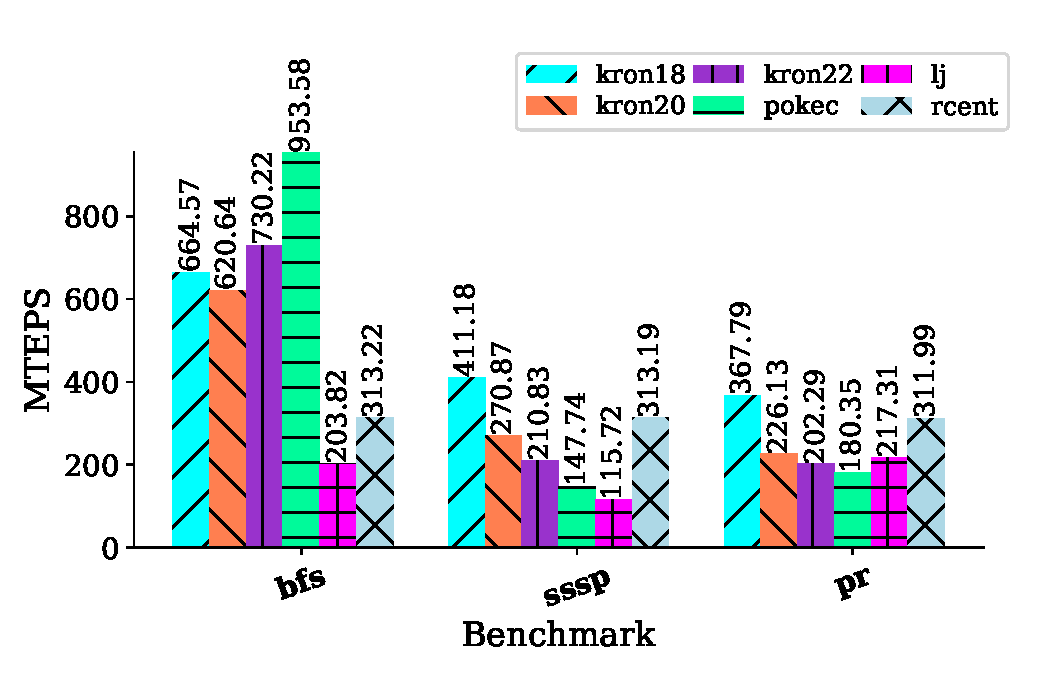
\includegraphics[scale = 0.5]{graphit-figures/baseline.pdf}
%     \caption{Baseline code generation results for each benchmark in the dense pull direction with no manycore specific optimizations.}
%     \label{pap:generals:sec:eval:fig:baseline}
% \end{figure}
% }

% \newcommand{\pushEvalFigure}{
% \begin{figure}[t]
%     \centering
%     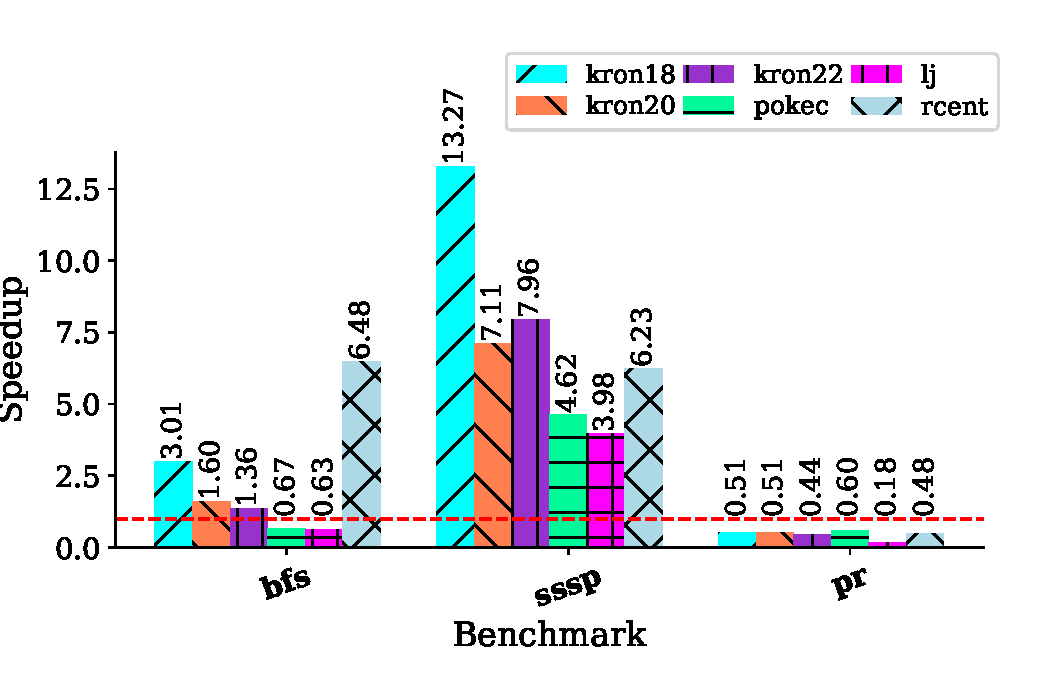
\includegraphics[scale = 0.5]{graphit-figures/push.pdf}
%     \caption{Baseline code generation results for each benchmark in the push direction with no manycore specific optimizations.}
%     \label{pap:generals:sec:eval:fig:push}
% \end{figure}
% }

% \newcommand{\edgeSpeedupFigure}{
% \begin{figure}[t]
%     \centering
%     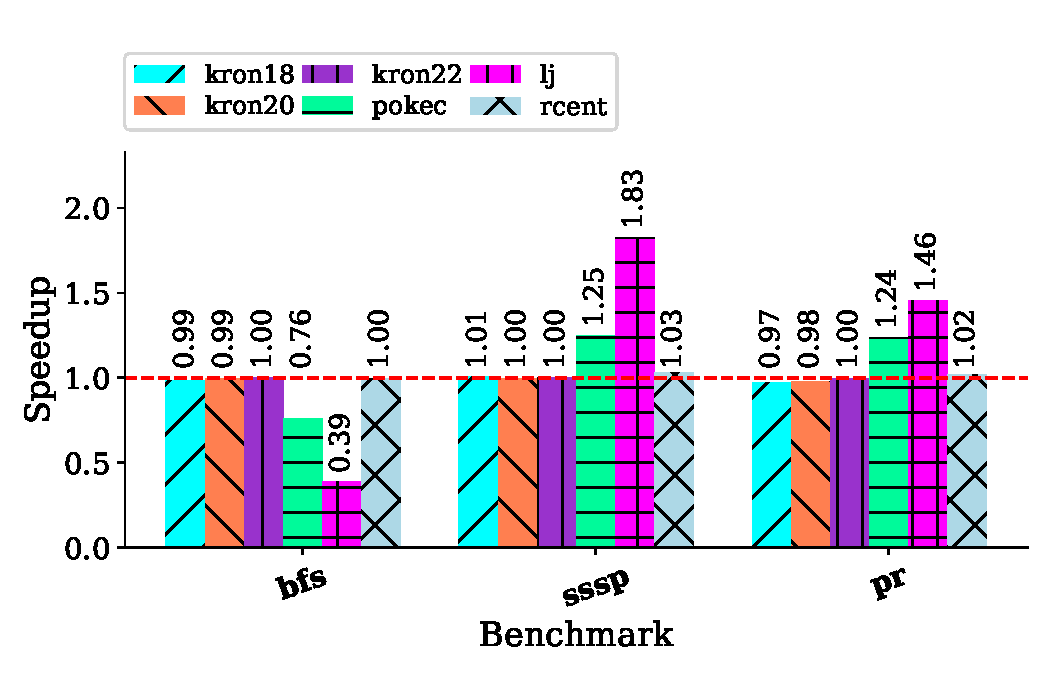
\includegraphics[scale = 0.5]{graphit-figures/edge.pdf}
%     \caption{Speedup results for edge based optimization over the baseline dense pull implementation for each benchmark.}
%     \label{pap:generals:sec:eval:fig:edge}
%     \vspace{-2mm} 
% \end{figure}
% }

\newcommand{\blockBFSFigure}{
\begin{figure}[t]
    \centering
    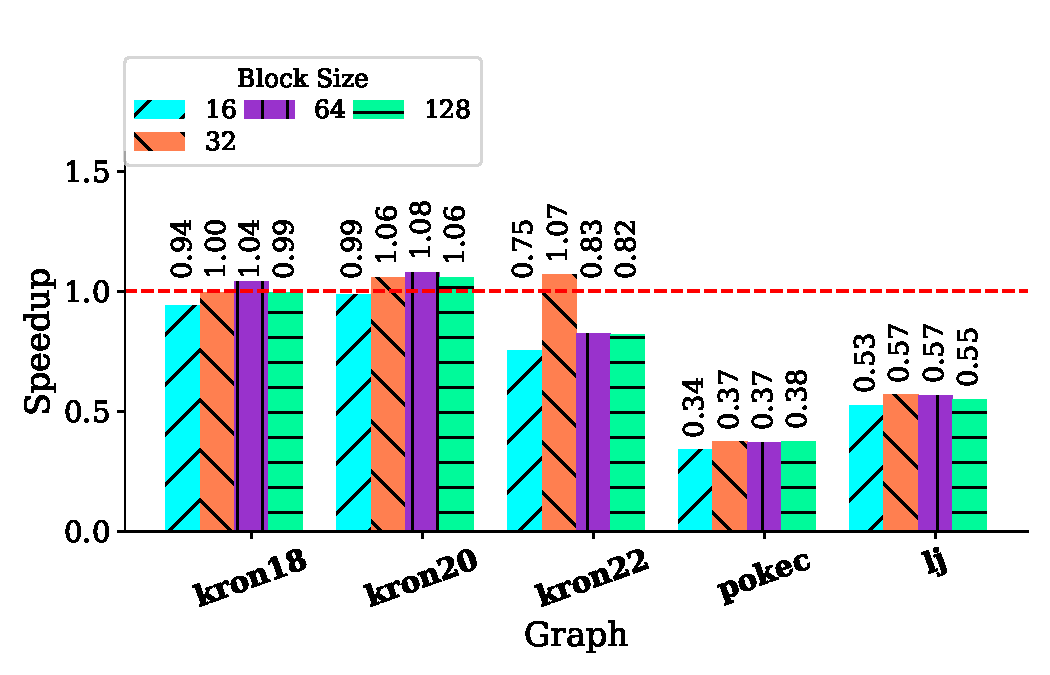
\includegraphics[scale = 0.5]{graphit-figures/bfs-block.pdf}
    \caption{MTEPS results for varying block sizes using the blocked access method on BFS.}
    \label{pap:generals:sec:eval:fig:bfsblock}
\end{figure}
}

\newcommand{\blockSSSPFigure}{
\begin{figure}[t]
    \centering
    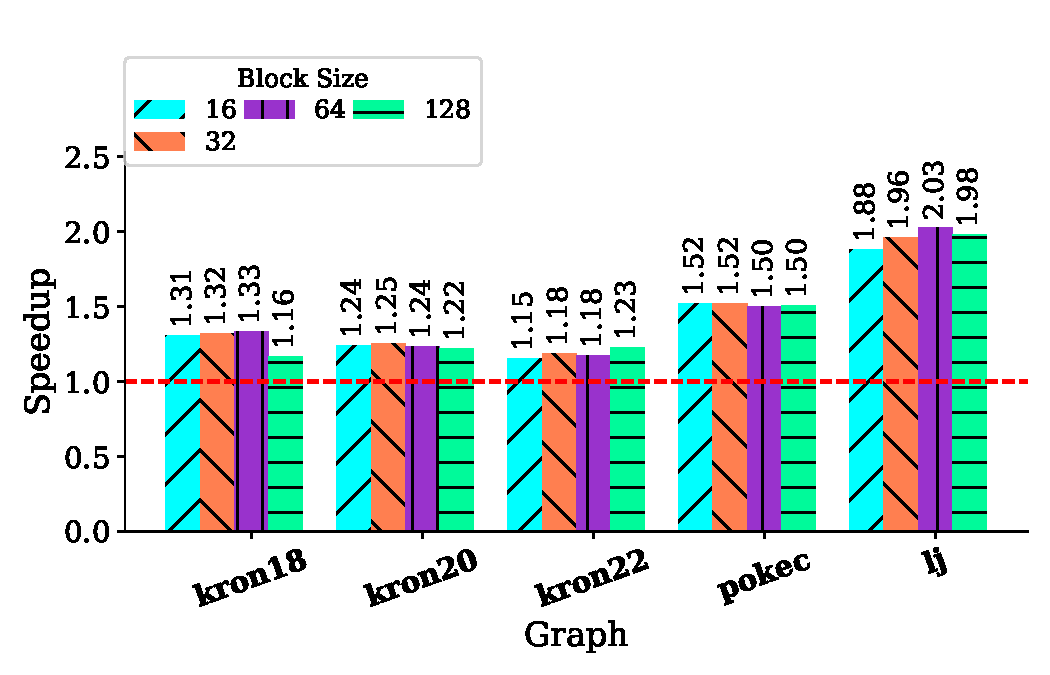
\includegraphics[scale=0.5]{graphit-figures/sssp-block.pdf}
    \caption{Speedup results for varying block sizes using the blocked access method on SSSP. Speedup is calculated over the baseline pull direction implementation.}
    \label{pap:generals:sec:eval:fig:ssspblock}
\end{figure}
}

\newcommand{\cacheBFSFigure}{
\begin{figure}[t]
    \centering
    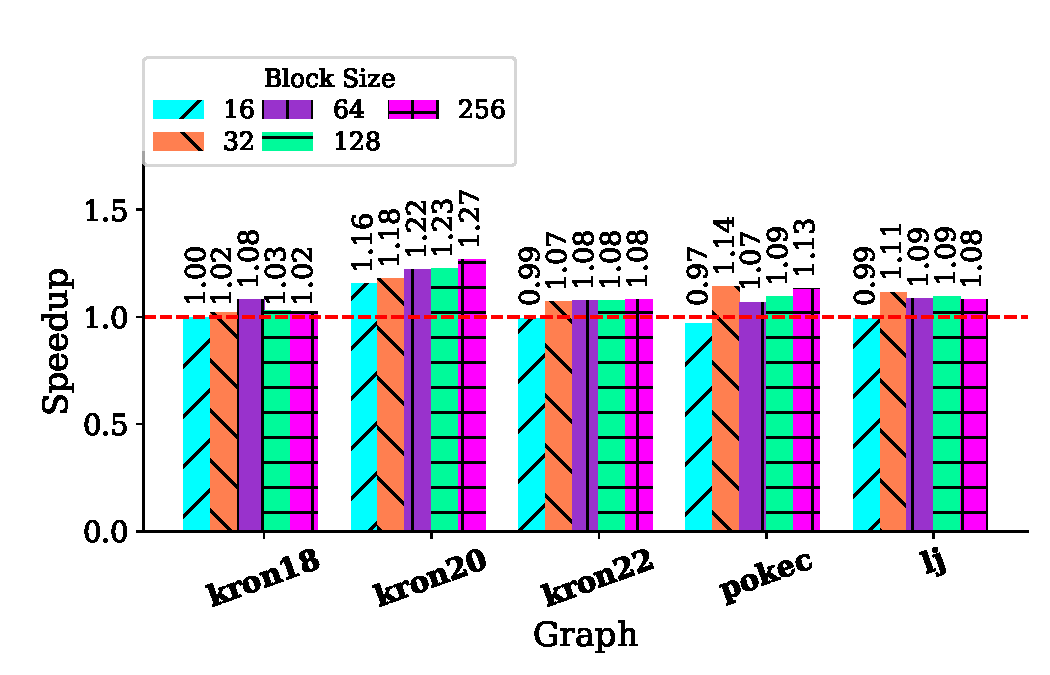
\includegraphics[scale = 0.5]{graphit-figures/bfs-cache.pdf}
    \caption{MTEPS results for varying work block sizes using the manycore aware vertex partitioning scheme on BFS.}
    \label{pap:generals:sec:eval:fig:bfscache}
\end{figure}
}

\newcommand{\cacheSSSPFigure}{
\begin{figure}[t]
    \centering
    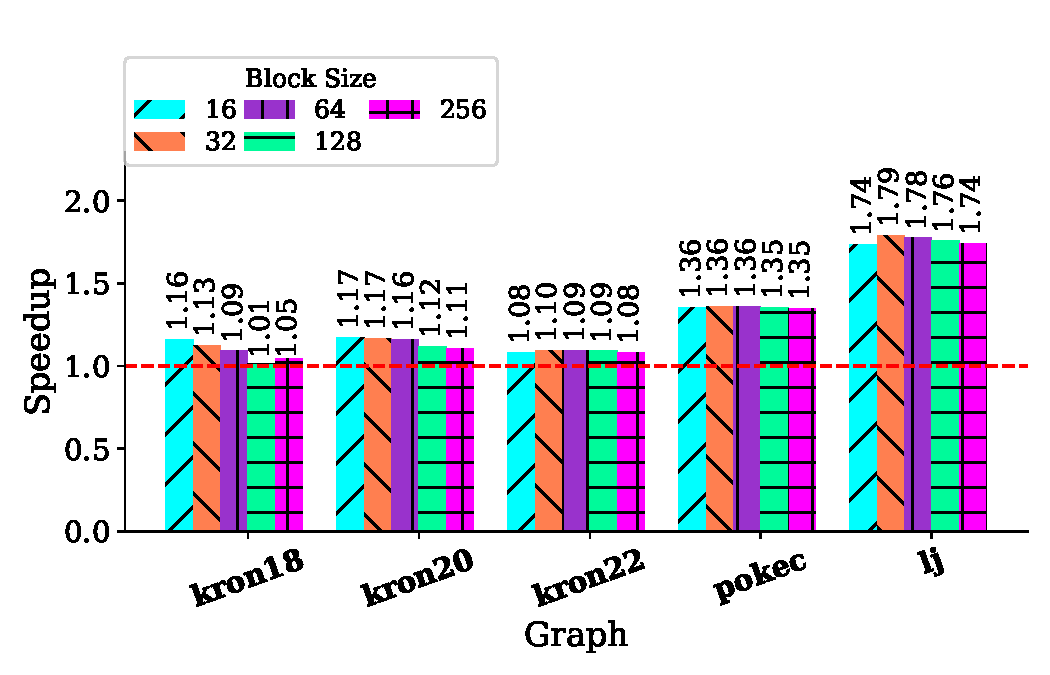
\includegraphics[scale=0.5]{graphit-figures/sssp-cache.pdf}
    \caption{Speedup results for varying work block sizes using the manycore aware vertex partitioning scheme on SSSP. Speedup is calculated over the baseline pull direction implementation.}
    \label{pap:generals:sec:eval:fig:ssspcache}
\end{figure}
}

% \newcommand{\allBlockedFigure}{
% \begin{figure}[t]
%     \centering
%     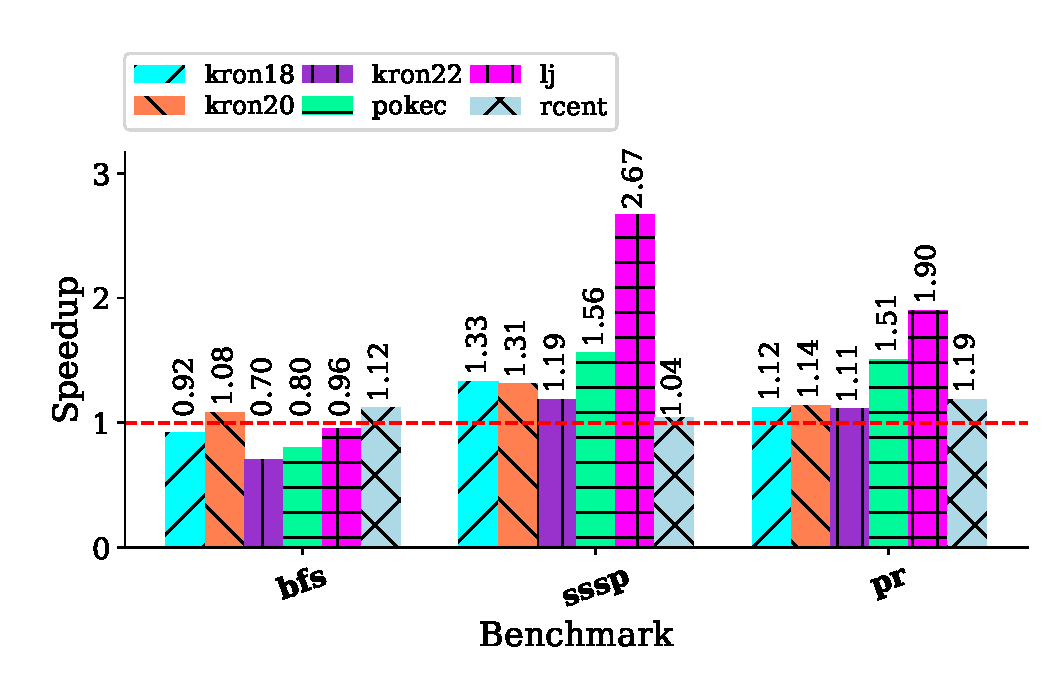
\includegraphics[scale = 0.5]{graphit-figures/all-blocked.pdf}
%     \caption{Blocked access method speedup results for each benchmark. Speedup is calculated over the baseline pull direction implementation.} %For each graph and benchmark, block sizes of 16, 32, 64, and 128 elements were tested and the best performing block size is reported here.
%     \label{pap:generals:sec:eval:fig:blocked}
% \end{figure}
% }

% \newcommand{\allAlignedFigure}{
% \begin{figure}[t]
%     \centering
%     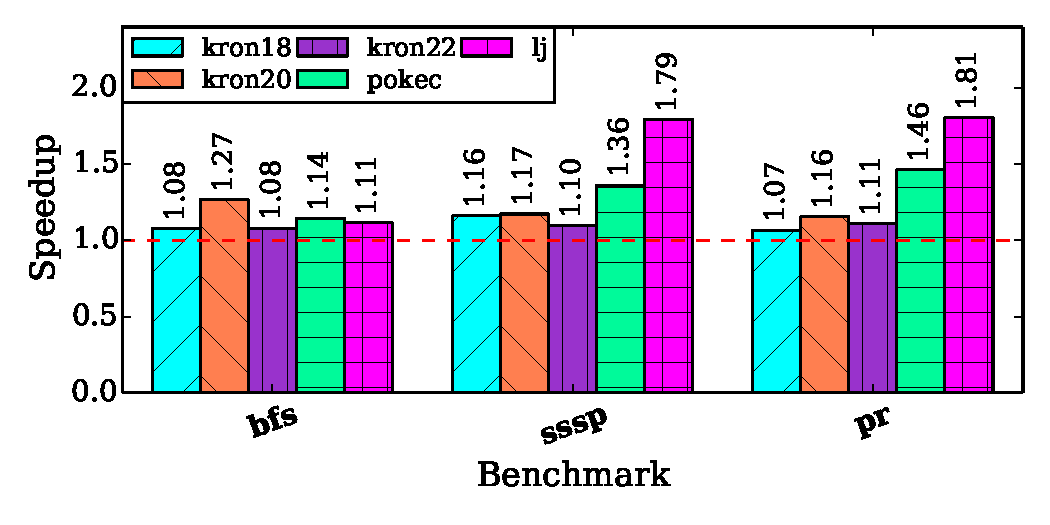
\includegraphics[scale = 0.5]{graphit-figures/align.pdf}
%     \caption{Alignment-based partitioning speedup results for each benchmark. Speedup is calculated over the baseline pull direction implementation.} %For each graph and benchmark, work group sizes of 16, 32, 64, 128, and 256 vertices were tested and the best performing work group size is reported here.
%     \label{pap:generals:sec:eval:fig:aligned}
%     \vspace{-2mm} 
% \end{figure}
% }

%I am not sure if this is the best way to present an overview of results or if we need it. 

\newcommand{\overviewResultsTable}{
    \begin{sidewaystable}
    \centering
    \begin{footnotesize}
    \begin{tabular}{llccccl}
    %\hline
        \toprule
        \textbf{Benchmark} & \textbf{Graph} & \textbf{Traversed Edges} & \textbf{Time (ms)} & \textbf{MTEPS} & \textbf{Speedup} & \textbf{Schedule}  \\ \midrule
        \multirow{ 6}{*}{BFS} & kron18 & 364,687 & 3.02 & 120.61 & 3.01 &\push \\ %\cline{2-7}
        & kron20 & 3,075,348 &19.82 & 155.13 & 1.60 & \push \\ %\cline{2-7}
        & kron22 & 130,762,502 & 136.73 & 956.38 & 1.38 & \hybrid \\ %\cline{2-7}
        & pokec & 28,787,299 & 32.60 & 916.15 & 3.74 & \hybrid, alignment-based partitioning on \pull \\ %\cline{2-7}
        & LJ  & 31,773,988 &  80.68  & 393.83 &  1.93 & \pull, alignment-based partitioning \\ %\cline{2-7}
        & road\_central  & 470 &  0.13  & 3.39 &  2342.51 & \push, bucketed sparse frontier\\ \hline
        \multirow{ 6}{*}{SSSP} &kron18  & 769,042 &  1.77  & 434.36 &  15.68 & \push \\ %\cline{2-7}
        & kron20  & 12,300,469 &  19.96  & 616.26&  8.7 & \push\\ %\cline{2-7}
        & kron22  & 86,836,312 &  155.19  & 559.51 &  5.89 & \push \\ %\cline{2-7}
        & pokec  & 10,018,259 &  236.91  & 42.29 &  2.62 & \push, bucketed sparse frontier \\ %\cline{2-7}
        & LJ  & 128,114,036 & 515.65  & 248.45 & 3.44 & \push, \\ %\cline{2-7}
        & road\_central  & 850 &  0.15  & 5.35 &  2043.07 & \push, bucketed sparse frontier\\ \hline
        \multirow{ 6}{*}{PR} & kron18  & 3,805,022 &  9.23  & 412.34 &  1.12 & \pull, blocked access method\\ %\cline{2-7}
        & kron20  & 15,700,369 &  60.07  & 261.35 &  1.16 & \pull, alignment-based partitioning\\ %\cline{2-7}
        & kron22  & 64,155,711 &  285.29  & 224.88 &  1.11 & \pull, blocked access method\\ %\cline{2-7}
        & pokec  & 30,622,564 &  112.34  & 272.58 &  1.51 & \pull, blocked access method\\ %\cline{2-7}
        & LJ  & 34,681,189 &  83.96  & 413.06 &  1.90 & \pull, blocked access method\\ %\cline{2-7}
        & road\_central  & 33,866,826 &  91.57  & 369.84 & 1.19 & \pull, blocked access method \\ %\hline
        \bottomrule
    \end{tabular}
    \end{footnotesize}
    \caption{Table containing best execution time results across all benchmarks and input graphs. The total number of traversed edges, achieved MTEPS, speedup over the baseline implementations, and the optimizations used to achieve these results are also listed above. Note that algorithmic changes can affect the total number of traversed edges. As a result, a benchmark may report speedup over the baseline but report lower overall MTEPS. This is especially noticeable on the road\_central graph as discussed in Section~\ref{sec:discussion}}
    \label{sec:eval:tab:summary}
    \end{sidewaystable}
}

\newcommand{\relatedMTEPSTable}{
\begin{table}
\centering
\begin{footnotesize}
\begin{tabular}{cllll}
%\hline
\toprule
 \textbf{Source} & \textbf{Platform} & \textbf{Benchmark} & \textbf{Graph}  & \textbf{MTEPS} \\ \midrule
 \cite{slota2015high}& Xeon Phi MIC & CC & LJ (22) & 240 \\ %\hline
 \cite{slota2015high}& Xeon Phi MIC & CC & Flickr (19) & 140\\ %\hline
 %Galois \cite{aasawat2018well}& Ivy Bridge & PR & LJ (22) & 207.67 \\ \hline
 \cite{khorasani2014cusha} & GTX780 & BFS & LJ (22) & 272.4 \\ %\hline
 \cite{zhong2013medusa}& C2050 & BFS & KKT (21) & 351.5 \\ %\hline
 \cite{yang2019graphblast}& k40c & SSSP & LJ (22) & 334.2 \\ %\hline
 \cite{wang2016gunrock} & k40c & SSSP & LJ (22) & 217.9 \\
 \bottomrule

\end{tabular}
\end{footnotesize}
\caption{Performance results in MTEPS from other graph processing frameworks. The benchmark CC is strongly connected components.}
\label{sec:related:tab:mteps}
\end{table}

}


% \newcommand{\graphInfoTable}{
% \begin{table}[]
% \centering
% \begin{tabular}{cccc}
% %\hline
% \toprule
%  \textbf{Name} & \textbf{Scale} & \textbf{\# Vertices} & \textbf{\# Edges} \\ \midrule %\hline
%  kron18 & 18 & 262,144 & 4,194,304 \\ %\hline
%  kron20 & 20 & 1,048,576 & 16,777,216 \\ %\hline
%  kron22 & 22 & 4,194,304 & 67,108,864 \\ %\hline
%  pokec & 20.5 & 1,632,803 & 30,622,564 \\ %\hline
%  livejournal (lj) & 22 & 3,997,962 & 34,681,189 \\ %\hline
%  \bottomruleå
% \end{tabular}


% \caption{The vertex and edge information for each of the graphs used in our evaluation. We use synthetic \kron graphs used in the Graph500 benchmark and two real world graphs.}
% \label{sec:eval:tab:graphs}
% \end{table}
% }